\documentclass[12pt]{article}
\usepackage[english]{babel}
\usepackage[utf8]{inputenc}
\usepackage[table,xcdraw]{xcolor}
\usepackage{graphicx}
\usepackage{listings}
\usepackage{hyperref}
\usepackage{vmargin}
\usepackage{wrapfig}
\usepackage{subfiles}
\usepackage{float}
\usepackage{amsmath}
\usepackage{multirow}

\title{Anàlisis - Processament Segmentat}
\author{Oriol Alàs Cercós i Marta Albets Mitjaneta}
\date{24 de Maig del 2019}

\setpapersize{A4}
\setmargins{2.5cm}  % margen izquierdo
{1.5cm}             % margen superior
{16.5cm}            % anchura del texto
{23.42cm}           % altura del texto
{10pt}              % altura de los encabezados
{1cm}               % espacio entre el texto y los encabezados
{0pt}               % altura del pie de página
{2cm}               % espacio entre el texto y el pie de página 

\def\contentsname{Índex}
\begin{document}
\begin{titlepage}
\begin{figure}[htb]
\begin{center}
	
\includegraphics[width=4cm]{imgs/UDL.png}
   	\vspace*{\stretch{1.0}}
   	\\
   	\medskip
   	\begin{center}
   		\noindent\rule{16.5cm}{0.4pt}
   		\linebreak 
   		\\
      	\Huge\textbf{Activitat d’Avaluació}
      	\\
      	\Large\textbf{Optimització de Consultes}
      	\noindent\rule{16.5cm}{0.4pt}
      	\\
      	\bigskip
      	\normalsize{Fet per:}
      	\\
      	\large\textit{Oriol Alàs Cercós},
      	\large\textit{Àiax Faura Vilalta},
      	\large\textit{Joan Martí Olivart},
      	\\
      	\setlength{\parskip}{1em}
      	\normalsize{Dia de termini:}
      	\\
      	\large{10 de Març 2020}
   	\end{center}
   	\vspace*{\stretch{2.0}}
\end{center}
\end{figure}
\begin{flushright}
	Universitat de Lleida
	\\
	Escola Politècnica Superior
	\\
	Grau en Enginyeria Informàtica
	\\
	Ampliació de Bases de Dades i Enginyeria del Programari
	\\
	\medskip
	\textbf{Professorat:}
	\\
	Juan Manuel Gimeno
\end{flushright}
\thispagestyle{empty} 
\end{titlepage}
\tableofcontents
\thispagestyle{empty}
\newpage
\renewcommand*\listfigurename{Índex de figures}
\listoffigures
\thispagestyle{empty}

\newpage
\setcounter{page}{1}
%\subfile{sections/introduction.tex}
\section{Exercici 1}
\textbf{Proposa un arbre equivalent a la següent consulta, calcula el volum de dades que es va tractant al llarg de tot l’arbre i fes la seva optimització sintàctica.}\\\\
L'arbre dissenyat equivalent a la consulta es pot veure a la figura \ref{fig:cons1}.
\begin{figure}[H]
	\centering
	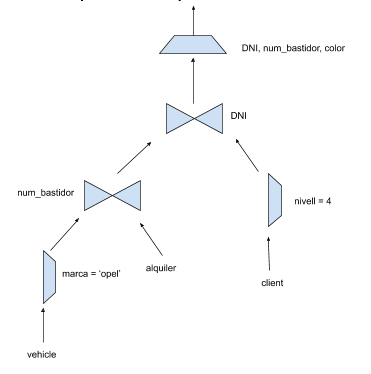
\includegraphics[width=8cm]{imgs/img1.png}
	\label{fig:cons1}
	\caption{Proposta d'arbre equivalent a la consulta}
\end{figure}
Un cop dissenyat, es realitzen els diferents passos a seguir.
\begin{enumerate}
	\item \textit{Baixar les seleccions}.
	Com es pot observar a la figura \ref{fig:cons1}, les seleccions estan en el nivell més baix possible.
	\item \textit{Reagrupar seleccions}. No hi ha seleccions a agrupar.
	\begin{figure}[H]
		\centering
		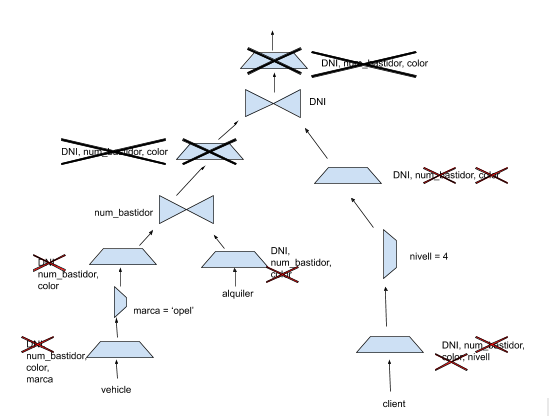
\includegraphics[width=8cm]{imgs/img2.png}
		\label{fig:consdos}
		\caption{Arbre un cop baixades les projeccions.}
	\end{figure}

	\begin{figure}[H]
		\centering
		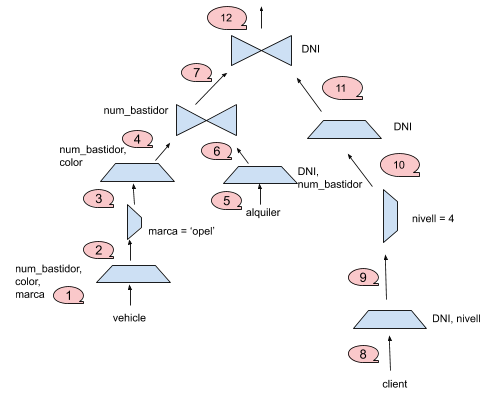
\includegraphics[width=8cm]{imgs/consnum.png}
		\label{fig:consre}
		\caption{Arbre sense les projeccions redundants.}
	\end{figure}
	\item \textit{Baixar projeccions}. 
	Un cop baixades les projeccions, hem tret tots aquells atributs que no es troben, tal i com s'observa a la figura \ref{fig:consdos}.
	\item El resultat un cop simplificant les projeccions, treient aquelles que no realitzen cap tipus de canvi es pot veure a la figura 3.

\end{enumerate}
\subsection{Càlcul del volum de dades}
\begin{figure}[H]
	\centering
	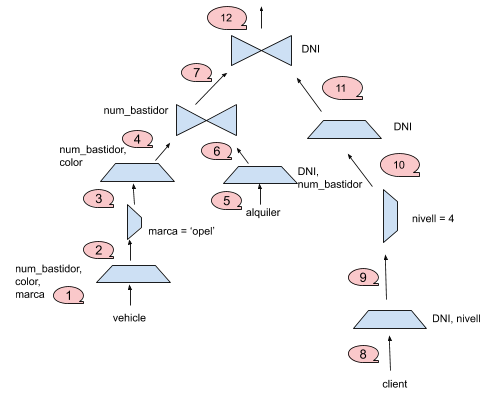
\includegraphics[width=8cm]{imgs/consnum.png}
	\label{fig:consnum}
	\caption{Arbre amb els diferents passos que segueix la selecció.}
\end{figure}
Per indicar que la cardinalitat d’un pas fa referència a un pas anterior, s’ha indicat el nombre del pas al que fa referència subrallant-lo. Exemple: card(6) = cardinalitat que es tenia en el pas 6.
\begin{enumerate}
	\item 
	card(vehicle) = 50\\
	mida(vehicle) = 3 +15 +15 + 5 = 38\\
	volum = 50 x 38 = 1900
	\item 	card(1) = 50\\					
	mida =  3 + 15 + 5 = 23\\				
	volum = 50 x 23 = 1150	
	\item card(2) = 50 x 0,2 = 10			\\	
	mida = 23						\\
	volum = 10 x 23 = 230	
	\item card(3) = 10						\\
	mida = 3 + 5 = 8					\\
	volum = 10 x 8 = 80		
	\item card(alquiler) = 50					\\
	mida(alquiler) = 3 + 3 + 6 = 12			\\
	volum = 50 x 12 = 600	
	\item card(5) = 50						\\
	mida = 3 + 3 = 6					\\
	volum = 50 x 6 = 300		
	\item card(max(4,6)) = card(6) = 50 \\
				mida = 8 + 6 - 3 = 11\\
				volum = 50 x 11 = 550
	\item card(client) = 250\\
	mida =  3 + 30 + 15 + 3 = 51				\\
	volum = 250 x 51 = 12750				
	\item card(8) = 250 \\
	mida = 3 + 3 = 6\\
	volum = 250 x 6 = 1500
	\item card(9) = 250 x 0.25\\
	mida = 6\\
	volum = 63 x 6 = 378
	\item card(10) = 63\\
	mida = 3\\
	volum = 63 x 3 = 189
	\item card(max(7,11)) = card(11) = 63\\
	mida = 11 + 3 - 3 = 11\\
	volum = 63 x 11 = 693
	
\end{enumerate}
Total = 1900 + 1150 + 230 + 80 + 600 + 300 + 550 + 12750 + 1500 + 378 + 189 + 693
Total  = 20320

\section{Exercici 2}
\textbf{Descriu dues estratègies d’execució per a resoldre la següent consulta, tot indicant les possibles combinacions d’algorismes d’implementació de cada operació segons que cada algorisme, per a cada operació, sigui o no aplicable. 
\\\\
Cal deixar indicada, mitjançant la fòrmula i les dades corresponents, l’estimació de costos en les opcions aplicables (no poseu simplement el resultat final) i justificar (1 línia) l’aplicabilitat o no de l’algorisme. }\\
\subsection{Estratègia A}
Selecció de la relació alquiler i després fer el join d’alquiler i vehículo i després seleccionar la relació segons l’atribut marca provinent de vehículo.
\subsubsection{Selecció de la relació alquiler}
\begin{itemize}
\item 1r Algorisme: No realitzable ja que fecha-devolución no és índex cluster
\item 2n Algorisme: No realitzable ja que fecha-devolución no és índex cluster
\item 3r Algorisme: No realitzable ja que fecha-devolución no és índex no cluster
\item 4t Algorisme: Lectura seqüencial.
\[cost = B_{alquiler}=3\]
\item 5è Algorisme: No realitzable ja que fecha-devolución no és índex no cluster
\item 6è Algorisme: No realitzable perquè la relació no està en diferents fitxers.
\item 7è Algorisme; No realitzable perquè fecha-devolución no és índex cluster.
\end{itemize}

Per tant, l’algorisme òptim per realitzar la consulta és el 4t.
\subsubsection{Guardar la selecció}
Es busca la cardinalitat de la selecció:
\[card(seleccio) = card(alquiler) * percentatge_{fecha-devolucion > ‘21-2-2020’}=50*\frac{35}{100}=17.5 \simeq 18
\]
Per tal de trobar el nombre de blocs de la selecció, s’ha de trobar el factor de bloqueig, que és:
\[b_{alquiler}= \frac{mida_{pagina}}{mida_{tupla}}= \frac{50}{3}=16.6 \simeq 17\]
\[B_{alquiler}= \frac{card(seleccio)}{b_{alquiler}}= \frac{17.5}{17} \simeq 2\]
\subsubsection{Join vehículo - selecció alquiler}
\begin{itemize}
	\item \textbf{Bucles imbricats}. Com que es vol que el bucle amb menys iteracions sigui l’exterior:
	\[cost = B_{seleccio}+ B_{seleccio}*B_{vehicle} =2 + 2 * 10 = 22\]
	\item \textbf{Ordenació-fusió}. La relació vehicle ja està ordenada per \textit{numbastidor}, doncs aquesta és la seva clau primària. Llavors, només s’ha de tenir en compte que la selecció no està ordenada per aquest atribut.
	\[cost =2*log_2(B_{seleccio})*B_{seleccio}+2*log_2(B_{vehicle})*B_{vehicle}+B_{seleccio}+B_{vehicle}=\]
	\[= 2*log_2(B_{seleccio})*B_{seleccio}+B_{seleccip}+B_{vehicle}= 2 *log_2(2)*2+2+10=16\]
\item \textbf{Bucle amb índex}. Es pot aplicar perquè vehicle té l'índex cluster num-bastidor i està ordenat per aquest índex. Com a màxim, hi haurà 18 tuples que facin join, per tant, el cost d’aquest algorisme és: 
\[cost =B_{seleccio}+card(seleccio) +S*card(seleccio)*card(vehicle)= 2+17.5 +17.5 =37\]
\end{itemize}
Per tant, l'algorisme per realitzar el join és el d'ordenació-fusió.
\subsubsection{Cost total}
\[
cost_{Estrategia A}=3+2+16=21\]
\subsection{Estratègia B}
La segona estratègia seleccionada ha estat fer primer les seleccions i desprès la combinació (join entre ambdòs seleccions).
\subsubsection{Selecció de la relació vehículo}
\begin{itemize}
	\item 1r Algorisme: No realitzable ja que marca no és un índex cluster.
	\item 2n Algorisme: No realitzable ja que marca no és un índex cluster.
	\item 3r Algorisme. Realitzable ja que marca és un índex cluster i la selecció és de la forma $$ A_i = cte $$
	\[cost = S(marca = 'opel') * card(vehiculo) = \frac{card(vehiculo)}{NDIST(marca)} = \frac{50}{7} = 8\]
	\item 4t Algorisme. Lectura seqüencial. \[cost = B_{vehiculo} = 10\]
	\item 5è Algorisme. No realitzable ja que la selecció no és de la forma: $ A_i >=, <=, <, > $
	\item 6è Algorisme. No realitzable ja que la relació no està en diferents fitxers.
	\item 7è Algorisme. Combinació d'indexos. És igual que l'algorisme 3, ja que no més hi ha un índex de vehículo que intervingui amb la consulta.
\end{itemize}
Per tant, l'algorisme òptim per realitzar la consulta és el 3r.
\subsubsection{Selecció de la relació alquiler}
La selecció de la relació alquiler és el mateix que en l'estratègia A, així que l'algorisme òptim per realitzar la consulta és el 4t amb $ cost = 3 $
\subsubsection{Guardar les seleccions}
Per guardar les seleccions, hem de saber les cardinalitats de les consultes.
\[card(query_{vehiculo}= card(vehiculo) * percentatge_{marca='Opel'}=50*\frac{20}{100}=10\]
\[B_{Vehiculo}=\frac{card(vehiculo)}{b_{vehiculo}}\Rightarrow b_{vehiculo}=\frac{card(vehiculo}{B_{vehiculo}} = \frac{50}{10}=5\]
\[B_{query_{vehiculo}}=\frac{card(query_{vehiculo})}{b_{vehiculo}}=\frac{10}{5}=2\]
\[card(query_{alquiler}= card(alquiler) * percentatge_{fecha-devolucion > ‘21-2-2020’}=50*\frac{35}{100}=17.5 \simeq 18
\]
Per tant, el cost de guarda la query de vehicle és 2.
\[B_{alquiler}=\frac{card(alquiler)}{b_{alquiler}}\Rightarrow b_{alquiler}=\frac{card(alquiler}{B_{alquiler}} = \frac{50}{3}=17\]
\[B_{query_{vehiculo}}=\frac{card(query_{vehiculo})}{b_{vehiculo}}=\frac{18}{17}=2\]

Per tant, el cost de guarda la query de vehiculo és 2.
\[cost_{total} = 2 + 2 = 4\]
El cost total de guardar les dues seleccions és 4.
\subsubsection{Join de les dues seleccions}
\begin{itemize}
	\item \textbf{Bucles imbricats}. Com que qualsevol de les dues tenen el mateix nombre de blocs, no importa quin és el bucle exterior o interior.
	\[cost = B_R + B_R * B_S = 2+2*2= 6\]
	\item \textbf{Ordenació-fusió}. Com que cap de les dues estan ordenades, s'han de realitzar les ordenacions.
	\[cost =2*log_2(B_{R})*B_{R}+2*log_2(B_{S})*B_{S}+B_{R}+B_{S}=\]
	\[= 2 *log_2(2)*2+2 *log_2(2)*2+2+2=12\]
	\item \textbf{Bucle amb índex}. No realitzable perquè al realitzar les dues seleccions ja no es poden utilitzar els índexs.
\end{itemize}

Per tant, l'algorisme per realitzar el join és el de bucles imbricats, amb un cost de 6.
\subsubsection{Cost total}
\[cost_{EstrategiaB}=8+3+4+6=21\]
\end{document}
